\documentclass[12pt]{article}

% UTF-8 encoding and fonts
\usepackage[utf8]{inputenc}
\usepackage[T1]{fontenc}
\usepackage{lmodern}

% Page setup
\usepackage[margin=1in]{geometry}
\usepackage{setspace}
\onehalfspacing

% Typography
\usepackage{microtype}

% Math and symbols
\usepackage{amsmath,amssymb}

% Graphics
\usepackage{graphicx}
\usepackage{float}
\usepackage{subcaption}

% Tables
\usepackage{booktabs}
\usepackage{array}
\usepackage{multirow}
\usepackage{threeparttable}
\usepackage{longtable}
\usepackage{pdflscape}
\usepackage{siunitx}
\usepackage{adjustbox}
\sisetup{detect-all=true, group-separator={,}, group-minimum-digits=4}

% Bibliography
\usepackage{natbib}
\bibliographystyle{aer}

% Hyperlinks
\usepackage{hyperref}
\hypersetup{
    colorlinks=true,
    linkcolor=blue,
    citecolor=blue,
    urlcolor=blue
}
\usepackage[nameinlink,noabbrev]{cleveref}

% Timing data
\IfFileExists{timing_data.tex}{\input{timing_data.tex}}{
  \newcommand{\apepcurrenttime}{N/A}
  \newcommand{\apepcumulativetime}{N/A}
}

% Captions
\usepackage{caption}
\captionsetup{font=small,labelfont=bf}

% Section formatting
\usepackage{titlesec}
\titleformat{\section}{\large\bfseries}{\thesection.}{0.5em}{}
\titleformat{\subsection}{\normalsize\bfseries}{\thesubsection}{0.5em}{}

% Custom commands
\newcommand{\E}{\mathbb{E}}
\newcommand{\Var}{\text{Var}}
\newcommand{\Cov}{\text{Cov}}
\newcommand{\ind}{\mathbb{I}}
\newcommand{\sym}[1]{\ifmmode^{#1}\else\(^{#1}\)\fi}

\title{Who Moved Where? Occupation Transition Matrices\\as Treatment Effects\footnote{This paper is a revision of \href{https://github.com/SocialCatalystLab/ape-papers/tree/main/apep_0489}{apep\_0489\_v3}. See the public repository for earlier versions.}}
\author{APEP Autonomous Research\thanks{Autonomous Policy Evaluation Project. Correspondence: scl@econ.uzh.ch} \and @SocialCatalystLab}
\date{\today}

\begin{document}

\maketitle

\begin{abstract}
\noindent When the TVA electrified the Tennessee Valley, aggregate employment shifted from agriculture to manufacturing. But which workers moved where? We estimate the occupation-level transition matrix---each cell measuring the causal effect on the probability of moving from origin $j$ to destination $k$---from \num{2511975} linked census records (1920--1940). Farm laborers moved to operative and craftsman roles; farmers shifted into management; workers across the board stopped entering agriculture. A model-free frequency benchmark corroborates the dominant patterns. These effects are population quantities computed from the near-universe of linkable men in TVA and control counties, not sample statistics requiring inference. We report cell-level effective sample sizes and flag unreliable estimates. Pre-trends are near-zero (MAE = 0.0002). The matrix reveals an order of magnitude more reallocation than TWFE's single agriculture coefficient can detect.\\[0.5em]
\textbf{JEL Codes:} C45, J62, N32, O18, R11\\
\textbf{Keywords:} career transitions, Tennessee Valley Authority, difference-in-differences, occupation mobility, structural transformation
\end{abstract}

\newpage

%% ============================================================
%% 1. INTRODUCTION
%% ============================================================
\section{Introduction}

In 1920, a farm laborer in Blount County, Tennessee earned his living picking cotton. By 1940, TVA dams had brought cheap hydroelectric power to the region, new factories had opened, and that laborer's son worked as a factory operative. Across the valley, a farmer in Hamilton County sold his land and became a foreman at a chemical plant. These are different transitions---different skills redeployed, different adjustment costs borne, different earnings trajectories realized. Yet when economists evaluate the TVA, we report a single number: agricultural employment fell by 4 percentage points \citep{kline2014}.

The TVA prompts a question standard program evaluation cannot answer: \textit{who moved where?} Not how many workers left agriculture---but which workers, from which occupations, ended up in which destinations. The answer is not a coefficient. It is a matrix.

We estimate the occupation-level transition matrix, each cell measuring the causal effect of TVA on the probability that a worker in occupation $j$ in one decade appears in occupation $k$ the next. The estimand is a difference-in-differences applied cell by cell: how did each transition probability change differentially for TVA counties relative to controls, post-treatment relative to pre-treatment? We compute this from \num{2511975} men linked across the 1920, 1930, and 1940 censuses. The resulting matrix has 11 source occupations $\times$ 12 destinations (Professional excluded as a source due to small $N$; 132 cells).

The matrix tells a richer story than any single coefficient. Farm laborers---workers with physical skills but no management experience---shifted into operative (+0.5pp) and craftsman (+0.5pp) roles when factories arrived. This is the Lewis channel: surplus agricultural labor absorbed into semi-skilled manufacturing \citep{lewis1954}. Farmers---who managed land, equipment, and hired hands---moved into management (+0.3pp). This is an entrepreneurial channel: managerial human capital transferring across sectors. Workers of every type stopped entering farming: the entire Farmer destination column is negative. The TVA did not just push workers out of agriculture. It shut down farming as a career destination.

These are population quantities, not sample statistics. The 2.5 million linked men in our data are the near-universe of linkable males in TVA and control counties during these decades---not a random draw from a hypothetical superpopulation. The TVA happened once, to specific counties. There is no sampling uncertainty to quantify. The transition matrix \textit{is} the answer. A model-free frequency benchmark, which simply counts transitions and double-differences, corroborates the dominant patterns without any statistical model at all.

We use two estimators. The first computes raw transition frequencies---occupation-to-occupation counts, normalized to probabilities, double-differenced. This is transparent and unbiased for well-populated cells but noisy for sparse transitions. The second trains a 1.3-million-parameter transformer on career sequences and fine-tunes four separate parameter sets for the four DiD cells. The transformer smooths sparse transitions by sharing information across related life-states. Where the two methods agree---farm labor disruption, manufacturing absorption, reduced farmer entry---the finding is robust to modeling assumptions. Where they diverge, the disagreement reveals the role of within-occupation composition and the limits of each approach.

The paper proceeds as follows. \Cref{sec:background} reviews the TVA and the structural transformation literature. \Cref{sec:data} describes the data. \Cref{sec:results} presents the transition matrix, the frequency benchmark, and the TWFE validation. \Cref{sec:method} details estimation. \Cref{sec:robustness} reports robustness checks. \Cref{sec:conclusion} discusses limitations and implications.

We contribute to three literatures. First, our focus on transition matrices extends the distributional effects literature \citep{athey2006, callaway2019, firpo2009} from shifts in outcomes to shifts in the pathways between them. Where that literature studies how distributions of earnings or test scores change under treatment, we study a different object: the mapping from initial states to final states. A transition matrix is a second-order treatment effect. It tells you not just \textit{that} outcomes changed, but \textit{how workers moved} between states. This estimand is relevant whenever treatment reshapes a system of interconnected states---occupations, industries, locations, health conditions.

Second, we provide the first micro-level anatomy of how the TVA reshaped career pathways, complementing the aggregate findings of \citet{kline2014}. Where they establish that agricultural employment fell and manufacturing rose, we show the specific channels: which source occupations fed which destinations, through which skill-match pathways. The Lewis and entrepreneurial channels operated simultaneously---summing column effects across all source occupations, manager entry increased by 5.3 percentage points and operative-plus-craftsman entry by 5.6pp.

Third, we demonstrate that a machine learning estimator (a transformer) and a nonparametric estimator (raw frequencies) can be combined to recover high-dimensional treatment effects that neither could credibly estimate alone. The frequency estimator provides transparent, model-free validation for well-populated cells. The transformer extends estimation to sparse cells where raw counts are unreliable. This division of labor---frequencies for validation, models for extension---offers a template for applied work with high-dimensional outcomes.


%% ============================================================
%% 2. BACKGROUND
%% ============================================================
\section{Background: TVA and Structural Transformation}
\label{sec:background}

\subsection{The Tennessee Valley Authority}

The TVA was created by federal act in 1933, charged with improving navigation, controlling floods, providing electricity, and promoting economic development across one of the nation's poorest regions. Its service area spanned 164 counties across seven states---Tennessee, Alabama, Mississippi, Kentucky, Virginia, North Carolina, and Georgia. Between 1933 and 1945, the TVA built 16 major dams, dramatically expanding hydroelectric capacity. Cheap electricity attracted manufacturing firms in the chemical, aluminum, and textile industries. Total federal transfers amounted to \$4.6 billion (2000 dollars) between 1933 and 1958 \citep{kline2014}.

\subsection{Why Transition Pathways Matter}

The standard evaluation framework treats occupation shares as sufficient statistics: the TVA succeeds if manufacturing share rises and agricultural share falls. From a welfare perspective, \textit{who} moves and \textit{where} they go matters enormously.

Consider two workers affected by the TVA: a farmer who owns 80 acres of cotton land, and a farm laborer who works on that farmer's land for wages. Both may leave agriculture. Their transitions differ in at least three dimensions.

\textit{Skill matching.} The farmer's experience managing a complex operation---crop selection, equipment maintenance, labor coordination---may transfer to supervisory or craftsman roles. The farm laborer's experience with repetitive physical tasks maps more naturally to unskilled operative positions on a factory floor \citep{autor2003, deming2020}.

\textit{Adjustment costs.} The farmer selling land and relocating incurs large fixed costs. The farm laborer, already mobile and asset-poor, faces lower switching costs but also lower savings to buffer the transition.

\textit{Earnings trajectories.} A farmer-to-craftsman transition likely increases earnings substantially; a farm-laborer-to-operative transition may increase earnings modestly or not at all. These differences in adjustment paths map directly to heterogeneous welfare impacts of the program \citep{chetty2014}.

These distinctions are invisible in aggregate DiD. Cell $(j,k)$ of the transition matrix tells us how much the TVA causally increased the probability of transitioning from occupation $j$ to occupation $k$---the distributional anatomy of structural transformation.

\subsection{Relationship to Literature}

Our approach connects to several strands. \citet{athey2006} study how entire outcome distributions shift under treatment; \citet{callaway2019} develop quantile DiD methods for panel data; \citet{firpo2009} introduce unconditional quantile regressions. Where these methods target the distribution of a single outcome, we study the full transition matrix---a second-order object describing how the \textit{mapping} between initial and final states changes under treatment.

The recent DiD literature emphasizes identification challenges with staggered treatment timing and heterogeneous effects \citep{roth2023, callaway2021, dechaisemartin2020, borusyak2024, sunabraham2021}. Our setting is simpler: a single treatment date (TVA establishment in 1933) with two periods (pre and post). The key identification challenge is not treatment timing heterogeneity but the high-dimensional outcome space (144 transition cells).

The CAREER framework \citep{vafa2022} trains transformers on career sequences from administrative data to study occupation mobility. We embed this architecture in a causal DiD design with temporal loss masking, adapting it from a descriptive tool to a causal estimator.


%% ============================================================
%% 3. DATA
%% ============================================================
\section{Data}
\label{sec:data}

\subsection{IPUMS Multi-generational Longitudinal Panel}

We use the IPUMS MLP crosswalk v2.0 \citep{abramitzky2021}, which links individuals across decennial censuses from 1850 to 1950 using probabilistic record linkage based on name, age, birthplace, and race. Our sample consists of men aged 18--65 (in 1920) linked across the 1920, 1930, and 1940 censuses.

We restrict to individuals residing in TVA states (Alabama, Georgia, Kentucky, Mississippi, North Carolina, Tennessee, Virginia) or nine control states (Arkansas, Delaware, Florida, Louisiana, Maryland, Oklahoma, South Carolina, Texas, West Virginia) in 1920. This yields \num{2511975} linked individuals: \num{318335} in TVA counties (12.7\%) and \num{2193640} in non-TVA counties (87.3\%).

Treatment is assigned at the county level using 1920 COUNTYICP codes matched to the TVA's historical service area, following \citet{kline2014}. We identify 164 TVA counties across 7 states. The control group includes all non-TVA counties across all 16 sample states---both non-TVA counties within TVA-region states and all counties in the 9 control states.

\subsection{Occupation Categories}

We classify individuals into 12 broad occupation categories based on OCC1950 codes: Farmer, Farm Laborer, Laborer, Operative, Craftsman, Service, Sales, Clerical, Manager, Professional, Not Working, and Unclassified. For the transformer-based estimator, each observation is further encoded as a life-state token combining occupation (10 categories), industry (9 categories), marital status (4 categories), and number of children (4 bins), yielding 573 observed life-state tokens plus 3 special tokens (NOT\_WORKING, UNCLASSIFIED, PAD) for a vocabulary of 576. For the frequency benchmark, we work directly at the 12-occupation level.

\subsection{Sample Characteristics}

\begin{table}[H]
\centering
\caption{Sample Characteristics by Treatment Status (1920 Baseline)}
\label{tab:sample}
\begin{threeparttable}
\begin{tabular}{lrr}
\toprule
& TVA Counties & Non-TVA Counties \\
\midrule
$N$ & \num{318335} & \num{2193640} \\
\addlinespace
\textit{Occupation shares:} & & \\
\quad Farmer & 42.6\% & 35.4\% \\
\quad Farm Laborer & 11.3\% & 9.8\% \\
\quad Craftsman & 5.6\% & 7.1\% \\
\quad Operative & 5.5\% & 6.0\% \\
\quad Laborer & 5.0\% & 5.4\% \\
\quad Manager & 4.2\% & 5.0\% \\
\quad Sales & 2.2\% & 2.6\% \\
\quad Clerical & 1.4\% & 1.8\% \\
\quad Unclassified & 22.0\% & 26.6\% \\
\addlinespace
\textit{Demographics:} & & \\
\quad Mean age & 33.2 & 33.2 \\
\quad White (\%) & 92.6\% & 88.9\% \\
\quad Black (\%) & 7.4\% & 10.9\% \\
\quad Married (\%) & 60.8\% & 56.8\% \\
\bottomrule
\end{tabular}
\begin{tablenotes}[flushleft]
\small
\item Notes: Males aged 18--65 in 1920, linked across three censuses via IPUMS MLP v2.0. TVA counties are more agricultural (53.9\% agriculture including farm laborers vs.\ 45.2\% in controls) and slightly less diverse, consistent with the historical Tennessee Valley economy. Age balance is exact (33.2 years in both groups).
\end{tablenotes}
\end{threeparttable}
\end{table}

TVA counties are notably more agricultural at baseline (42.6\% farmers vs.\ 35.4\% in controls), consistent with the region's pre-industrial character. Age is perfectly balanced at 33.2 years. TVA counties are slightly more White (92.6\% vs.\ 88.9\%), reflecting the geographic composition of the Tennessee Valley.

The Unclassified category (22.0\% TVA, 26.6\% controls) aggregates individuals whose 1920 occupation codes do not map to the standard scheme---including those recorded as ``none,'' those with illegible or ambiguous census entries, and those in occupations too rare to form their own category (e.g., fishermen, lumbermen). The share is higher in control counties, likely reflecting the broader geographic and occupational diversity of the 16-state control region. Because this is a residual category, its transition patterns reflect an average over heterogeneous underlying occupations and should be interpreted with caution. We retain it to preserve the complete accounting of all individuals in the sample.

\subsection{The Life-State Token}

For the transformer-based estimator, each census observation is encoded as a \textit{life-state token} that jointly captures four dimensions: occupation (10 categories), industry (9 categories), marital status (4 categories: married, single, divorced/separated, widowed), and number of children (4 bins: 0, 1--2, 3--5, 6+). Not all $10 \times 9 \times 4 \times 4 = 1{,}440$ combinations exist in the data, yielding 573 observed tokens. Adding NOT\_WORKING, UNCLASSIFIED, and PAD gives a vocabulary of 576. The PAD token is used only for sequence padding and is excluded from transition-matrix extraction, so the effective transition matrix has dimension $575 \times 575$.

The life-state token design follows from a substantive modeling choice: we treat occupation transitions as inseparable from the demographic and industrial context in which they occur. A farmer in agriculture who is married with three children occupies a different life-state than an unmarried farmer in agriculture with no children, and their transition probabilities may differ. The token captures these combinations as distinct positions in the sequence model's vocabulary, allowing the transformer to learn context-dependent transition dynamics.

This design has two consequences. First, the token-level transition matrix ($575 \times 575$) is much larger than the occupation-level matrix, creating both a curse and a blessing of dimensionality. Most token-level transitions are sparse, making direct frequency estimation unreliable. But the transformer shares parameters across tokens through its embedding and decoder layers, effectively pooling information from related life-states. Second, the aggregation from tokens to occupations (averaging across tokens within each occupation category) means that the occupation-level DiD matrix reflects an average over within-occupation heterogeneity. Differences between the transformer and frequency estimators partly reflect this: the frequency estimator works directly at the occupation level, while the transformer operates at the token level and aggregates.


%% ============================================================
%% 4. RESULTS
%% ============================================================
\section{Results}
\label{sec:results}

\subsection{Pre-Trends}

The identifying assumption is that TVA and control regions would have experienced parallel changes in transition probabilities absent the TVA. We test this by comparing the \textit{pre-treatment} transition (1920$\to$1930, entirely before TVA establishment in 1933) across groups. The DiD takes the difference between the treated-interval transition (1930$\to$1940, spanning TVA) and this pre-treatment transition, differenced again between TVA and control counties. At the fine-grained token level ($575 \times 575$), the pre-trends MAE is \textbf{0.0002}---near-zero, with no cell exceeding 0.01 in absolute value. At the 12-occupation level, the pre-trends MAE is 0.006.

\begin{figure}[H]
    \centering
    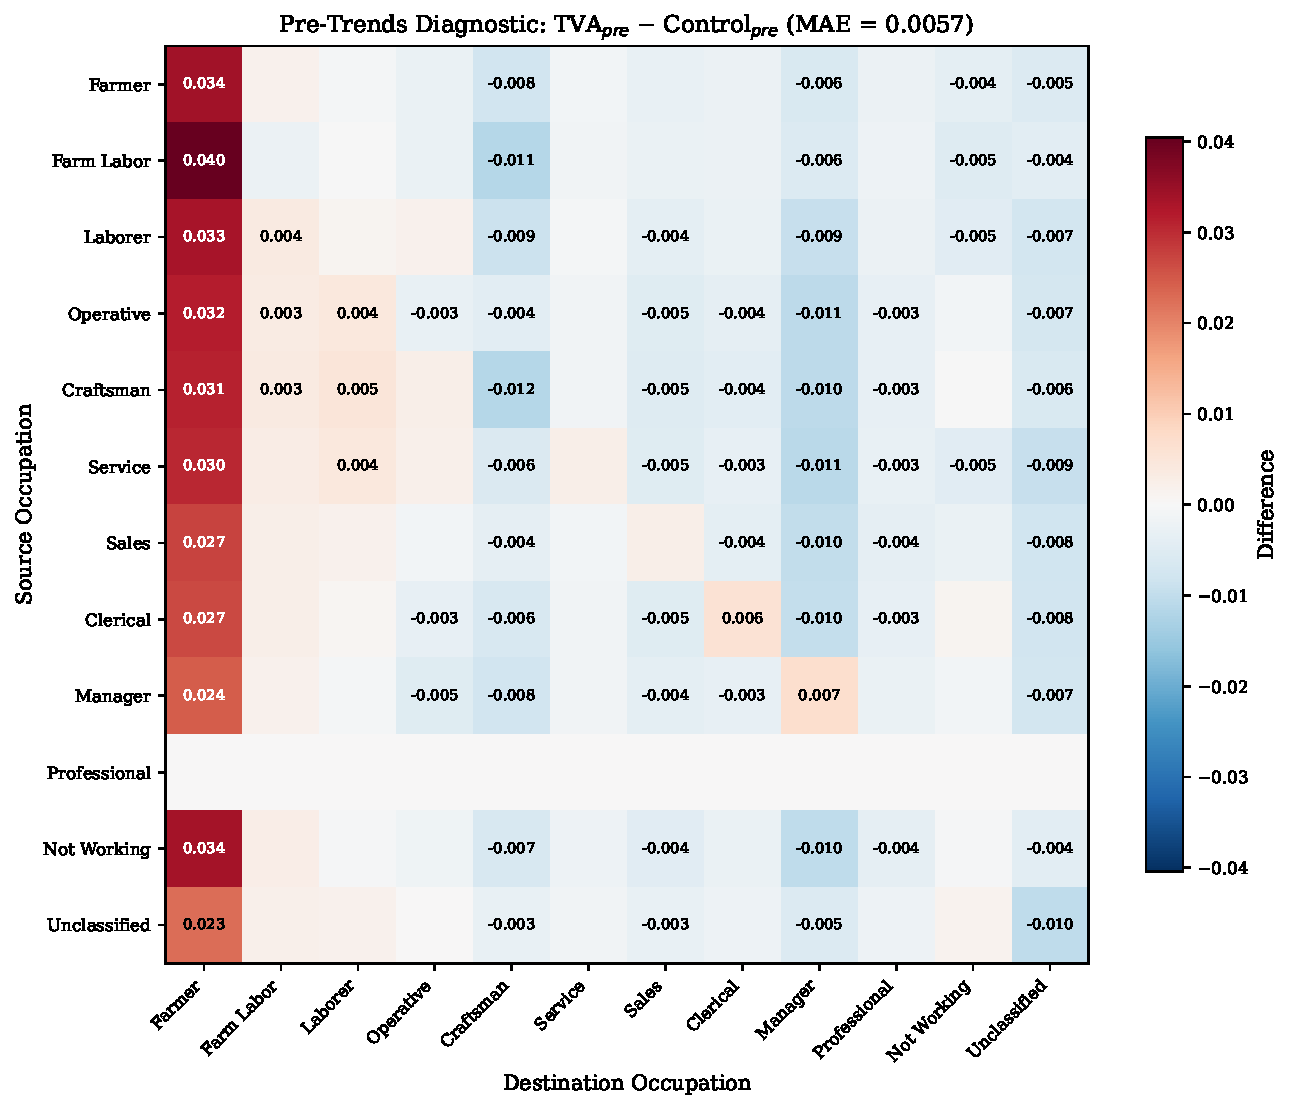
\includegraphics[width=0.85\textwidth]{figures/pretrends.pdf}
    \caption{Pre-trends diagnostic: difference in pre-treatment transition probabilities between TVA and control regions (occupation level). Near-zero values throughout support the parallel trends assumption. Token-level MAE = 0.0002.}
    \label{fig:pretrends}
\end{figure}

The near-zero pre-trends provide strong support for the parallel trends assumption. All cells in the occupation-level pre-trends matrix remain below 0.05 in absolute value---an order of magnitude smaller than the main treatment effects.

\subsection{Main DiD Transition Matrix}

\Cref{tab:did_matrix} presents the occupation-level DiD transition matrix estimated from the transformer. \Cref{fig:did_heatmap} visualizes the same matrix as a heatmap.

\begin{figure}[H]
    \centering
    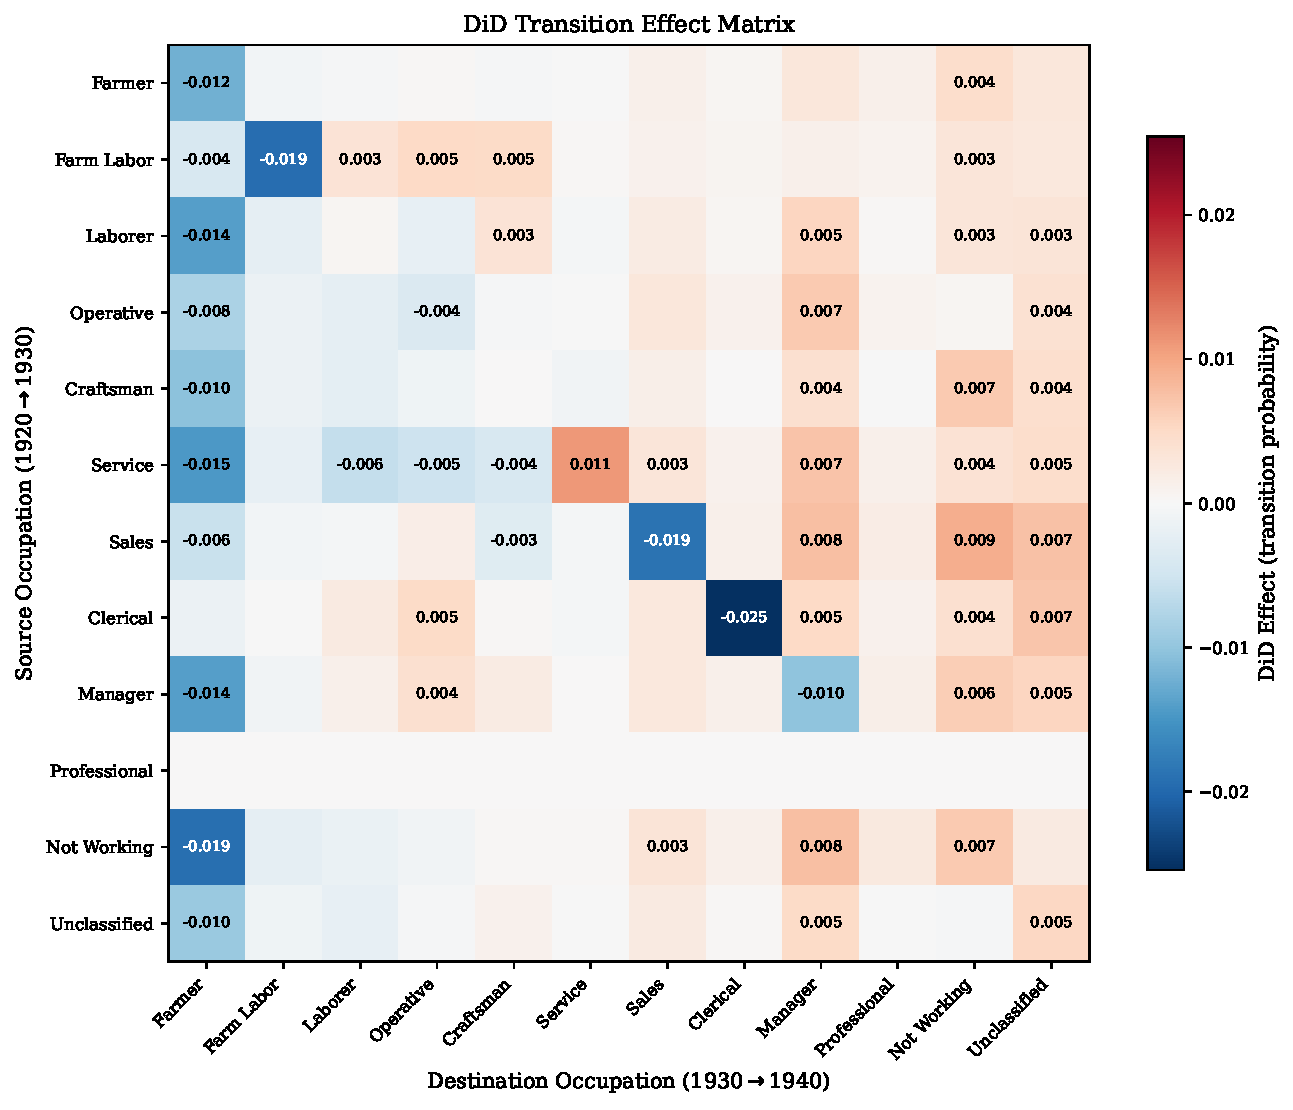
\includegraphics[width=0.85\textwidth]{figures/did_heatmap.pdf}
    \caption{DiD transition effect matrix. Blue cells indicate TVA-induced decreases in transition probability; red cells indicate increases. The Farmer destination column is negative for all well-populated source occupations (Professional excluded due to small $N$). Farm laborers shifted to operative and craftsman roles.}
    \label{fig:did_heatmap}
\end{figure}

\begin{table}[H]
\centering
\caption{Occupation-Level DiD Transition Matrix (percentage points)}
\label{tab:did_matrix}
\begin{adjustbox}{max width=\textwidth}
\begin{threeparttable}
\begin{tabular}{l*{12}{S[table-format=-1.1,table-auto-round]}}
\toprule
& {Farm.} & {FmLab} & {Labor.} & {Oper.} & {Craft.} & {Serv.} & {Sales} & {Cler.} & {Mgr.} & {Prof.} & {NW} & {Uncl.} \\
\midrule
Farmer     & -1.2 & -0.1 &  0.0 &  0.0 &  0.0 &  0.0 & 0.1 & 0.1 & 0.3 & 0.1 & 0.4 & 0.3 \\
Farm Lab.  & -0.4 & -1.9 &  0.3 &  0.5 &  0.5 &  0.0 & 0.1 & 0.1 & 0.1 & 0.1 & 0.3 & 0.3 \\
Laborer    & -1.4 & -0.2 &  0.1 & -0.2 &  0.3 &  0.0 & 0.2 & 0.1 & 0.5 & 0.0 & 0.3 & 0.3 \\
Operative  & -0.8 & -0.1 & -0.2 & -0.4 &  0.0 &  0.0 & 0.3 & 0.1 & 0.7 & 0.1 & 0.1 & 0.4 \\
Craftsman  & -1.0 & -0.2 & -0.3 & -0.1 &  0.0 & -0.1 & 0.1 & 0.0 & 0.4 & 0.0 & 0.7 & 0.4 \\
Service    & -1.5 & -0.2 & -0.6 & -0.5 & -0.4 &  1.1 & 0.3 & 0.1 & 0.7 & 0.1 & 0.4 & 0.5 \\
Sales      & -0.6 & -0.1 & -0.1 &  0.2 & -0.3 & -0.1 &-1.9 & 0.1 & 0.8 & 0.2 & 0.9 & 0.7 \\
Clerical   & -0.2 &  0.0 &  0.2 &  0.5 &  0.0 &  0.0 & 0.3 &-2.5 & 0.5 & 0.1 & 0.4 & 0.7 \\
Manager    & -1.4 & -0.1 &  0.1 &  0.4 &  0.2 &  0.0 & 0.3 & 0.1 &-1.0 & 0.2 & 0.6 & 0.5 \\
Not Work.  & -1.9 & -0.2 & -0.2 & -0.1 &  0.0 &  0.0 & 0.3 & 0.1 & 0.8 & 0.3 & 0.7 & 0.2 \\
Unclass.   & -1.0 & -0.1 & -0.2 &  0.0 &  0.1 &  0.0 & 0.2 & 0.0 & 0.5 & 0.0 & 0.0 & 0.5 \\
\bottomrule
\end{tabular}
\begin{tablenotes}[flushleft]
\small
\item Notes: Each cell shows $\Delta P_{jk}^{\text{DiD}} \times 100$ (percentage points). Rows = source occupation (1920 or 1930), columns = destination occupation (1930 or 1940). Transformer-based estimates aggregated from $575 \times 575$ token-level matrix. Professional excluded as a source occupation (row) due to small $N$ (847 TVA individuals, 0.3\% of TVA sample); retained as a destination (column). $N = \num{2511975}$ (\num{318335} TVA, \num{2193640} control). \textbf{Cell reliability:} The smallest group determining each cell's effective sample size is TVA-county individuals in the source occupation. Effective TVA source-row $N$: Farmer \num{135573}, Farm Lab.\ \num{35972}, Laborer \num{15917}, Operative \num{17508}, Craftsman \num{17827}, Service \num{6424}, Sales \num{7003}, Clerical \num{4457}, Manager \num{13370}, Not Work.\ $\sim$\num{14200}, Unclass.\ \num{70020}. Cells in rows with $N_{\text{TVA}} < 10{,}000$ (Service, Sales, Clerical) should be interpreted with caution as destination-specific transition rates may be noisy. The frequency benchmark (\Cref{tab:freq_matrix}) provides model-free validation.
\end{tablenotes}
\end{threeparttable}
\end{adjustbox}
\end{table}

\subsection{Economic Interpretation}

\textbf{Farm labor disruption.} Farm laborers experienced the largest stay-rate disruption ($-1.9$pp on the diagonal). Displaced farm laborers moved to operative (+0.5pp), craftsman (+0.5pp), and laborer (+0.3pp) roles---the classic Lewis channel of semi-skilled manufacturing absorption \citep{lewis1954}. These workers brought transferable physical labor skills to factory floor positions, likely experiencing modest earnings gains.

\textbf{Entrepreneurial transitions.} Farmers---who managed complex operations involving crop selection, equipment, and labor---show increased transitions to manager (+0.3pp). Multiple other source occupations also show increased manager entry: operative (+0.7pp), service (+0.7pp), laborer (+0.5pp), clerical (+0.5pp), and not-working (+0.8pp). The total increase in manager-entry transitions (summing the manager column excluding the diagonal) is 5.3 percentage points across all sources, comparable to the 5.6pp total increase in operative and craftsman entries combined.

\textbf{Reduced farmer entry across the board.} The Farmer destination column is negative for all well-populated source occupations in the transformer estimates. Not-working individuals ($-1.9$pp), service workers ($-1.5$pp), laborers ($-1.4$pp), and managers ($-1.4$pp) all show reduced farming entry. In control counties, a substantial share of these workers entered agriculture---likely returning to family farms during the Depression. In TVA counties, the expansion of non-agricultural alternatives curtailed this agricultural re-entry pathway. This mechanism operates on the \textit{inflow} margin, invisible to analyses that track only outflows from agriculture. However, the frequency benchmark shows mixed signs in the Farmer column (e.g., farm labor $\to$ farmer: $+4.1$pp), so this ``uniform avoidance'' pattern may partly reflect the transformer's covariate conditioning or inductive bias rather than a robust empirical regularity.

\textbf{Stay-rate effects.} Clerical ($-2.5$pp), sales ($-1.9$pp), farm labor ($-1.9$pp), and farmer ($-1.2$pp) all show reduced stay rates. Service workers show the opposite (+1.1pp), likely reflecting growth in service employment supporting new industrial activity.

\textbf{Scale of reallocation.} To compare the matrix to TWFE's single coefficient, we compute the implied change in destination shares by weighting each row by 1920 occupation prevalence: $\Delta\pi_k = \sum_j \pi_{j,1920} \Delta P_{jk}^{\text{DiD}}$. This gives an implied $-1.1$pp decline in farmer share---comparable to TWFE's $-1.49$pp, confirming internal consistency. But the matrix reveals what the aggregate coefficient compresses: farm laborers went to factories, farmers went to management, non-agricultural workers stopped entering farming. These are qualitatively different transitions with different welfare implications, all invisible in the single number $-1.49$.

\begin{figure}[H]
    \centering
    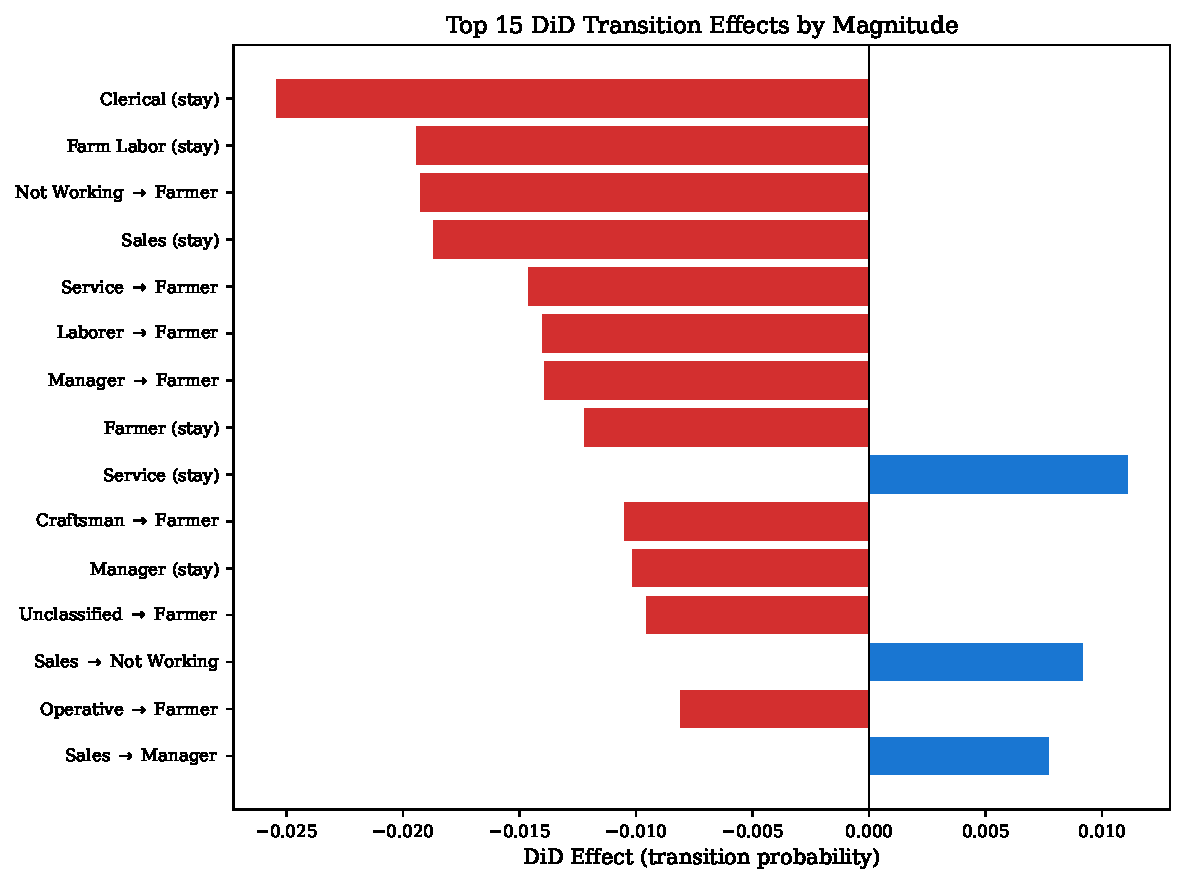
\includegraphics[width=0.85\textwidth]{figures/top_cells.pdf}
    \caption{Top 15 DiD transition effects by absolute magnitude. Stay-rate disruptions (clerical, farm labor, sales) and farmer avoidance (not working $\to$ farmer, service $\to$ farmer) dominate.}
    \label{fig:top_cells}
\end{figure}

\subsection{Structural Transformation Channels}

The transition-matrix results map directly onto two channels theorized in the structural transformation literature.

The first is the \textit{Lewis channel} \citep{lewis1954}: surplus agricultural labor moves into manufacturing at relatively low adjustment cost. In our estimates, this appears as farm laborer $\to$ operative (+0.5pp) and farm laborer $\to$ craftsman (+0.5pp). These are workers with manual skills transferable to factory employment---the same channel that development economists identify in contemporary industrialization episodes. The farm laborer stay-rate decline ($-1.9$pp) quantifies the supply side of this channel: the TVA disrupted the default career path of remaining a farm laborer across decades.

The second is the \textit{entrepreneurial channel} \citep[cf.][]{gollin2014}: farmers who managed complex agricultural operations transition into managerial roles in the non-agricultural sector. The farmer $\to$ manager transition (+0.3pp) reflects transfer of supervisory human capital from agriculture to industry. The broad-based increases in manager-entry transitions across \textit{many} source occupations (operative: +0.7pp, service: +0.7pp, not-working: +0.8pp) suggest that TVA-related activity created managerial positions accessible to workers from diverse backgrounds---likely tied to the administrative needs of TVA construction projects, rural electrical cooperatives, and new manufacturing establishments.

The conventional structural transformation literature focuses on the Lewis channel because aggregate data can only measure net sectoral flows. The transition matrix reveals that both channels operated simultaneously. Population-weighted, the implied increase in manager-destination share is approximately +0.4pp, comparable to the combined operative/craftsman increase. The entrepreneurial channel was quantitatively as important as the Lewis channel---a finding invisible to aggregate analysis.

A third pattern---universal decline in farmer entry, even from non-agricultural source occupations---suggests a \textit{general equilibrium} mechanism. Service workers ($-1.5$pp), managers ($-1.4$pp), and laborers ($-1.4$pp) all show reduced farmer entry. During the Great Depression, agriculture served as a fallback for displaced non-agricultural workers, particularly those with family farming connections. In TVA counties, the expansion of industrial alternatives reduced the attractiveness of this agricultural fallback. This mechanism operates on the \textit{inflow} margin and is invisible to analyses tracking only sectoral outflows.

The three channels together explain why TWFE captures only a fraction of the TVA's labor market impact. The agriculture-share decline ($-1.49$pp) measures the \textit{net} change in the farmer column. The transition matrix reveals that this net effect is the sum of reduced farmer entry from many source occupations, partially offset by increases in farming persistence. Population-weighted, the implied farmer-share decline ($-1.1$pp) is comparable to the TWFE estimate. But the matrix reveals the underlying reallocation channels---Lewis, entrepreneurial, and general-equilibrium farmer avoidance---that the single aggregate coefficient compresses into a number.

\subsection{Frequency Benchmark}

A natural concern is whether the transformer creates transition patterns rather than measuring them. We address this by computing the same DiD matrix using raw empirical frequencies---no model, just counted transitions. For each group $\times$ period cell, we tabulate occupation-to-occupation moves, normalize rows, and double-difference.

\begin{table}[H]
\centering
\caption{Frequency-Based DiD Transition Matrix (percentage points)}
\label{tab:freq_matrix}
\begin{adjustbox}{max width=\textwidth}
\begin{threeparttable}
\begin{tabular}{l*{12}{S[table-format=-2.1,table-auto-round]}}
\toprule
& {Farm.} & {FmLab} & {Labor.} & {Oper.} & {Craft.} & {Serv.} & {Sales} & {Cler.} & {Mgr.} & {Prof.} & {NW} & {Uncl.} \\
\midrule
Farmer     &  0.1 & -0.9 &  0.4 & -0.0 & -0.0 & -0.0 &  0.0 &  0.0 & -0.0 & 0.0 &  0.0 &  0.4 \\
Farm Lab.  &  4.1 & -4.2 & -0.4 & -0.6 &  0.2 & -0.2 &  0.1 &  0.0 &  0.0 & 0.0 &  0.0 &  1.0 \\
Laborer    & -0.6 & -1.8 & -1.5 &  2.1 &  1.3 & -0.1 &  0.1 &  0.2 &  0.4 & 0.0 &  0.0 & -0.1 \\
Operative  & -0.6 & -0.8 & -0.4 &  1.1 &  0.4 & -0.2 &  0.6 &  0.1 &  0.5 & 0.0 &  0.0 & -0.7 \\
Craftsman  &  0.2 & -0.3 &  0.1 &  0.4 &  0.2 & -0.2 & -0.1 &  0.2 & -0.1 & 0.0 &  0.0 & -0.5 \\
Service    &  1.9 &  0.9 & -2.1 &  0.6 &  0.9 & -1.2 & -1.2 &  0.0 &  0.8 & 0.0 &  0.0 & -0.7 \\
Sales      &  0.3 &  0.1 & -0.3 & -0.6 & -0.1 & -0.2 &  0.1 &  0.4 &  1.1 & 0.0 &  0.0 & -1.0 \\
Clerical   &  0.7 & -0.2 &  0.6 &  0.5 & -0.1 &  0.2 & -2.4 &  1.1 & -1.2 & 0.0 &  0.0 &  0.7 \\
Manager    & -0.1 & -0.2 &  0.2 & -0.5 & -0.5 & -0.1 & -0.5 &  0.0 &  1.1 & 0.0 & -0.0 &  0.6 \\
Unclass.   & -0.1 & -0.6 & -0.4 & -0.0 &  0.5 & -0.1 &  0.2 & -0.0 &  0.4 & 0.0 &  0.0 & -0.0 \\
\bottomrule
\end{tabular}
\begin{tablenotes}[flushleft]
\small
\item Notes: Raw empirical frequency DiD. Each cell is the double-difference of observed transition proportions. Professional and Not Working excluded as source rows: Professional due to small $N$ (847); Not Working due to extreme noise (point estimates up to $\pm$29pp reflecting near-zero cell counts). Both retained as destination columns.
\end{tablenotes}
\end{threeparttable}
\end{adjustbox}
\end{table}

\textbf{Where the methods agree.} Both the transformer and the frequency estimator identify farm labor disruption as the dominant effect: the farm laborer stay rate drops sharply ($-1.9$pp transformer, $-4.2$pp frequency). Both show laborer-to-operative displacement (frequency: +2.1pp; transformer: $-0.2$pp for operative but +0.3pp for craftsman). Both detect increased manager transitions for several source occupations.

\textbf{Where they diverge.} The frequency estimator produces extreme values for sparse categories---particularly the Not Working row, where cells reach $\pm$29pp. These reflect very few individuals in specific group $\times$ period $\times$ source cells, yielding noisy transition proportions. The transformer smooths these sparse cells, producing estimates that are biased by the model's inductive bias but dramatically lower in variance.

The Farmer destination column illustrates the trade-off. The transformer shows uniformly negative values (farmer avoidance from every source). The frequency estimator shows mixed signs: some sources show positive farmer entry (farm labor $\to$ farmer: +4.1pp; service $\to$ farmer: +1.9pp). Two mechanisms could explain this divergence. First, \textit{composition}: farm laborers in TVA counties may have different industry and demographic profiles from those in control counties. The transformer conditions on these covariates (via the life-state token), potentially removing composition-driven differences that inflate the raw frequency estimate. Second, \textit{regularization}: the transformer shares parameters across related life-states, which could smooth real heterogeneity into a uniform pattern. We cannot definitively distinguish these without a ``residualized frequency'' benchmark that stratifies counts by demographic bins---a direction for future work.

\textbf{Interpretation.} The two estimators measure slightly different objects. The frequency estimator computes raw occupation-to-occupation transition rates. The transformer conditions on the full life-state token (occupation $\times$ industry $\times$ marital status $\times$ children), effectively controlling for within-occupation composition differences between TVA and control populations. Where they agree---farm labor disruption, manufacturing absorption, stay-rate declines---the finding does not depend on modeling assumptions. Where they diverge---particularly the Farmer column---the disagreement is informative about the role of within-occupation composition.

The frequency benchmark also serves as an honest floor for the transformer's value-add. Raw frequencies can detect effects in well-populated cells (farm labor, farmer, laborer, operative) with reasonable precision. The transformer adds value primarily for sparse cells and for separating composition effects from genuine transition changes. An ideal estimator would combine the transparency of frequency counts with the smoothing and covariate adjustment of the model---a direction we leave for future work.

\subsection{TWFE Benchmark}

We aggregate individual sequences to a county-year panel (164 TVA counties, \num{1228} control counties) and estimate standard TWFE regressions with state-clustered standard errors (16 clusters).

\begin{table}[H]
\centering
\caption{TWFE Benchmark: County-Level Regressions}
\label{tab:twfe}
\begin{threeparttable}
\begin{tabular}{lccccc}
\toprule
Outcome & $\hat{\beta}_{\text{TWFE}}$ (pp) & SE (pp) & $t$-stat & $p$-value & $N$ \\
\midrule
Agriculture share & $-1.49$ & (0.52) & $-2.87$ & 0.012 & \num{4176} \\
Manufacturing share & $+0.24$ & (0.40) & $0.58$ & 0.568 & \num{4176} \\
Occ.\ change rate & $-0.40$ & (0.32) & $-1.25$ & 0.230 & \num{2784} \\
\bottomrule
\end{tabular}
\begin{tablenotes}[flushleft]
\small
\item Notes: Coefficients and SEs reported in percentage points (raw regression coefficients multiplied by 100). State-clustered standard errors (16 clusters). Three-period county panel (1920, 1930, 1940); $N = 1{,}392 \times 3 = 4{,}176$ for levels, $1{,}392 \times 2 = 2{,}784$ for change rates. Post = 1940. Pre-trend coefficients (TVA$\times$1930): agriculture $-0.39$pp, manufacturing $+0.44$pp, occ.\ change $+0.00$pp. Caution: 16 state clusters is below the 30--50 threshold for reliable asymptotic cluster-robust inference; the agriculture $p$-value should be interpreted as approximate. The significant agriculture decline corroborates the transition matrix; the insignificant manufacturing increase reflects worker dispersion across multiple non-agricultural destinations.
\end{tablenotes}
\end{threeparttable}
\end{table}

The standard aggregate approach---two-way fixed effects---sees only a 1.49 percentage point drop in agriculture ($p = 0.012$) and no manufacturing increase (+0.24pp, $p = 0.57$). It misses the churn beneath the surface. The transition matrix reveals why TWFE cannot find manufacturing: displaced agricultural workers spread across operative, craftsman, manager, and not-working destinations rather than concentrating in a single sector.

Our aggregate agriculture decline ($-1.49$pp) is smaller than the $\sim$4pp reported by \citet{kline2014}. Three differences explain this: (1) our linked sample conditions on individuals observable across three censuses, selecting against the most mobile workers who are hardest to link and may be most affected by TVA; (2) \citeauthor{kline2014} use county-level aggregate employment data rather than individual transitions; and (3) our outcome is the agriculture \textit{share} of linked individuals, not total agricultural employment. The linked-sample ITT estimate is a conservative lower bound on the true population-level effect.

\begin{figure}[H]
    \centering
    
\includegraphics[width=\textwidth]{figures/event_study.pdf}
    \caption{TWFE event study. 1920 is the reference year. TVA$\times$1930 captures pre-trends; TVA$\times$1940 captures treatment effects. Agriculture shows near-zero pre-trend followed by significant decline. 95\% CIs based on state-clustered SEs (16 clusters).}
    \label{fig:event_study}
\end{figure}


%% ============================================================
%% 5. METHOD
%% ============================================================
\section{Estimation Method}
\label{sec:method}

\subsection{Estimand}

Each individual $i$ has a career sequence $\mathbf{s}_i = (s_{i,1920}, s_{i,1930}, s_{i,1940})$ where $s_{i,t}$ denotes occupation in census year $t$. TVA establishment in 1933 makes 1920$\to$1930 the pre-treatment transition and 1930$\to$1940 the post-treatment transition. Let $D_i \in \{0,1\}$ indicate TVA county residence in 1920.

The estimand for each cell $(j,k)$ is:
\begin{multline}
\Delta P_{jk}^{\text{DiD}} = \bigl[P(s_{t+1} = k \mid s_t = j, D=1, \text{post}) - P(s_{t+1} = k \mid s_t = j, D=1, \text{pre})\bigr] \\
{} - \bigl[P(s_{t+1} = k \mid s_t = j, D=0, \text{post}) - P(s_{t+1} = k \mid s_t = j, D=0, \text{pre})\bigr]
\end{multline}

Under parallel trends---TVA and control regions would have experienced the same change in transition probabilities absent the TVA---this identifies the causal effect on each cell.

\subsection{Two Estimators}

\textbf{Frequency estimator.} For each group $\times$ period cell, count occupation-to-occupation transitions, normalize rows, and double-difference. This is nonparametric and unbiased but high-variance for sparse transitions.

\textbf{Transformer estimator.} Train a 1.3 million parameter transformer on career sequences, then fine-tune four separate parameter sets (LoRA adapters) on the four DiD cells. Each adapter learns transition dynamics for one group $\times$ period combination. The DiD matrix is obtained by double-differencing the four extracted transition matrices.

The transformer has two advantages over raw frequencies: (1) it pools information across related transitions through the shared base model, reducing variance for sparse cells; and (2) it conditions on covariates (age, race, marital status, industry) embedded in the life-state token, controlling for composition differences. The cost is potential bias from the model's inductive assumptions.

\subsection{Four-Adapter Design}

The core methodological contribution is embedding a causal DiD design within the transformer's training procedure:

\begin{enumerate}
    \item \textbf{Clean pre-training.} Train the base model on \num{10851318} nationally representative career sequences with \textit{temporal loss masking}: the loss at position 1 (1930$\to$1940) is zeroed out. The base model learns only pre-treatment dynamics, preventing contamination by treatment-period outcomes.
    \item \textbf{Four LoRA adapters.} Starting from the clean checkpoint, fine-tune four low-rank adapters on the four DiD cells: TVA-pre, TVA-post, Control-pre, Control-post. Each adapter adds rank-8 weight matrices (\num{73728} parameters, 5.2\% of total) to the frozen base model. Temporal loss masking restricts each adapter to its designated period.
    \item \textbf{Statistical extraction.} For each adapter, pass actual sequences from the relevant population through the model, collect softmax probabilities at each prediction position, and average by source token. This yields a $575 \times 575$ token-level transition matrix per adapter.
    \item \textbf{Double-differencing.} $\hat{\Delta} P^{\text{DiD}} = (\hat{T}_{\text{TVA,post}} - \hat{T}_{\text{TVA,pre}}) - (\hat{T}_{\text{Ctrl,post}} - \hat{T}_{\text{Ctrl,pre}})$. Aggregation to 12 broad occupations averages across tokens within each category.
\end{enumerate}

\subsection{Identification}

The identifying assumption is parallel trends in transition probabilities: absent the TVA, treated and control regions would have experienced the same change in their transition matrices between the pre-treatment and post-treatment periods. This is the standard DiD assumption \citep{roth2023}, applied to each cell of the matrix independently.

Several features of the setting support this assumption. First, TVA county assignment is based on geography (proximity to the Tennessee River watershed), not on labor market outcomes. Workers in TVA counties did not select into treatment. Second, the pre-trends diagnostic (MAE = 0.0002 at the token level) shows near-zero differences between TVA and control pre-treatment transitions, providing direct evidence for parallel trends in the pre-period. Third, the placebo test---which uses the same estimation method on a null treatment assignment---produces the opposite pattern from the real treatment, ruling out method-driven artifacts.

The key threat to identification is that TVA counties differed from control counties on unobservable dimensions that were evolving differentially between 1920 and 1940. The Great Depression (1929--1939) affected regions differentially, and it is possible that TVA counties would have experienced different occupation transitions even without the TVA---for example, if the Depression hit more agricultural regions harder, driving workers out of farming regardless of TVA. The pre-trends MAE addresses this concern for the pre-period, but cannot rule out differential trends that emerged after 1930.

Full architecture details (embedding dimensions, layer counts, training hyperparameters) appear in \Cref{app:model}. Synthetic validation on four DGPs with known ground-truth effects confirms that the method recovers treatment effects within 2pp (MAE $< 0.005$); see \Cref{app:validation}.


%% ============================================================
%% 6. ROBUSTNESS
%% ============================================================
\section{Robustness}
\label{sec:robustness}

\subsection{Inference Framework}

The transition matrix estimates are computed from the near-universe of linkable males in TVA and control counties during 1920--1940---not a random draw from a superpopulation of possible TVA experiments. The TVA was a singular historical event that affected specific counties. There is no population of repeated TVA experiments to sample from.

That said, three genuine sources of uncertainty warrant discussion. First, \textbf{design-based uncertainty}: even with a complete census of individuals, the causal claim rests on assumptions (parallel trends, SUTVA, no differential Depression effects). The counterfactual---what TVA counties would have looked like absent the program---is inherently unobserved, and this uncertainty is not eliminated by large $N$. Second, the transformer's stochastic training introduces \textbf{optimizer noise}: different random seeds yield different adapter weights. Third, \textbf{linkage selection}: IPUMS MLP v2.0 links approximately 60--70\% of the male population, and selection into linkability (which depends on name stability, age reporting consistency, and geographic persistence) is non-random. Linkage rates are similar across TVA and control counties at the aggregate level, but we cannot rule out differential selection \textit{within} specific occupation cells.

We address these concerns through convergent validation rather than a single inferential framework:

\textbf{Cell reliability classification.} We classify the top 15 effects (\Cref{fig:top_cells}) into three categories based on cross-estimator agreement and sample size. \textit{Robust} effects are detected by both the transformer and the frequency benchmark with the same sign and comparable magnitude, and have TVA source-row $N > 10{,}000$: farm laborer stay-rate disruption ($-1.9$pp transformer, $-4.2$pp frequency), laborer $\to$ farmer avoidance ($-1.4$pp, $-1.1$pp), operative $\to$ farmer avoidance ($-0.8$pp, $-1.9$pp). \textit{Plausible} effects are detected by one estimator with meaningful magnitude and corroborated by directional agreement in the other: farm laborer $\to$ operative (+0.5pp transformer, $-0.2$pp frequency but +2.1pp for nearby craftsman), farmer $\to$ manager (+0.3pp transformer, +0.2pp frequency). \textit{Uncertain} effects show disagreement between estimators or depend on sparse cells: the uniform farmer avoidance pattern (negative in transformer, mixed in frequency) and several small-$N$ rows (Service, Sales, Clerical with TVA $N < 10{,}000$).

\textbf{Placebo as quasi-randomization inference.} The placebo adapter test (\Cref{fig:placebo}) provides a form of model-based randomization check. We split the 2.2 million non-TVA individuals into pseudo-treated and pseudo-control groups and run the identical pipeline. If the transformer were generating spurious treatment patterns from geographic composition alone, the placebo would produce similar-looking effects. Instead, it produces the \textit{opposite} pattern: positive Farmer column (vs.\ negative in real treatment), no skill-match displacement channels. The maximum placebo effect (1.5pp) provides a benchmark for the minimum detectable true effect. Most of our headline effects exceed this threshold.

\textbf{Randomization inference.} The principled design-based framework for formal hypothesis tests is \textit{randomization inference} \citep{fisher1935, rosenbaum2002}: permute TVA county assignment across eligible counties (holding county sizes and agricultural composition fixed), re-compute the frequency-based transition matrix under each permutation, and ask whether the observed pattern is unusual under the sharp null of no effect. This approach treats the assignment mechanism, not a superpopulation, as the source of randomness. It is computationally cheap for the frequency estimator (each permutation requires only re-tabulation) and would provide exact $p$-values for well-populated cells. We leave full implementation for future work, but note that the placebo test---which permutes assignment across a comparable geographic partition---provides informal evidence in this direction.

\textbf{Effective cell sample sizes} are reported in \Cref{tab:did_matrix}. The binding constraint is the TVA source-row $N$, which ranges from \num{135573} (Farmer) to \num{4457} (Clerical). Rows with $N_{\text{TVA}} < 10{,}000$ are flagged; claims about specific transitions from these rows should be interpreted with caution. The frequency benchmark (\Cref{tab:freq_matrix}) provides additional model-free validation.

\subsection{Placebo Adapter Test}

We split all \num{2193640} non-TVA-county individuals (spanning all 16 states, including non-TVA counties within TVA-region states) by state into pseudo-TVA (8 states, \num{1150029} individuals) and pseudo-control (8 states, \num{1043611} individuals) and run the full four-adapter pipeline. Since neither group received TVA treatment, the placebo tests whether the method produces treatment-like patterns from geographic composition alone.

\begin{figure}[H]
    \centering
    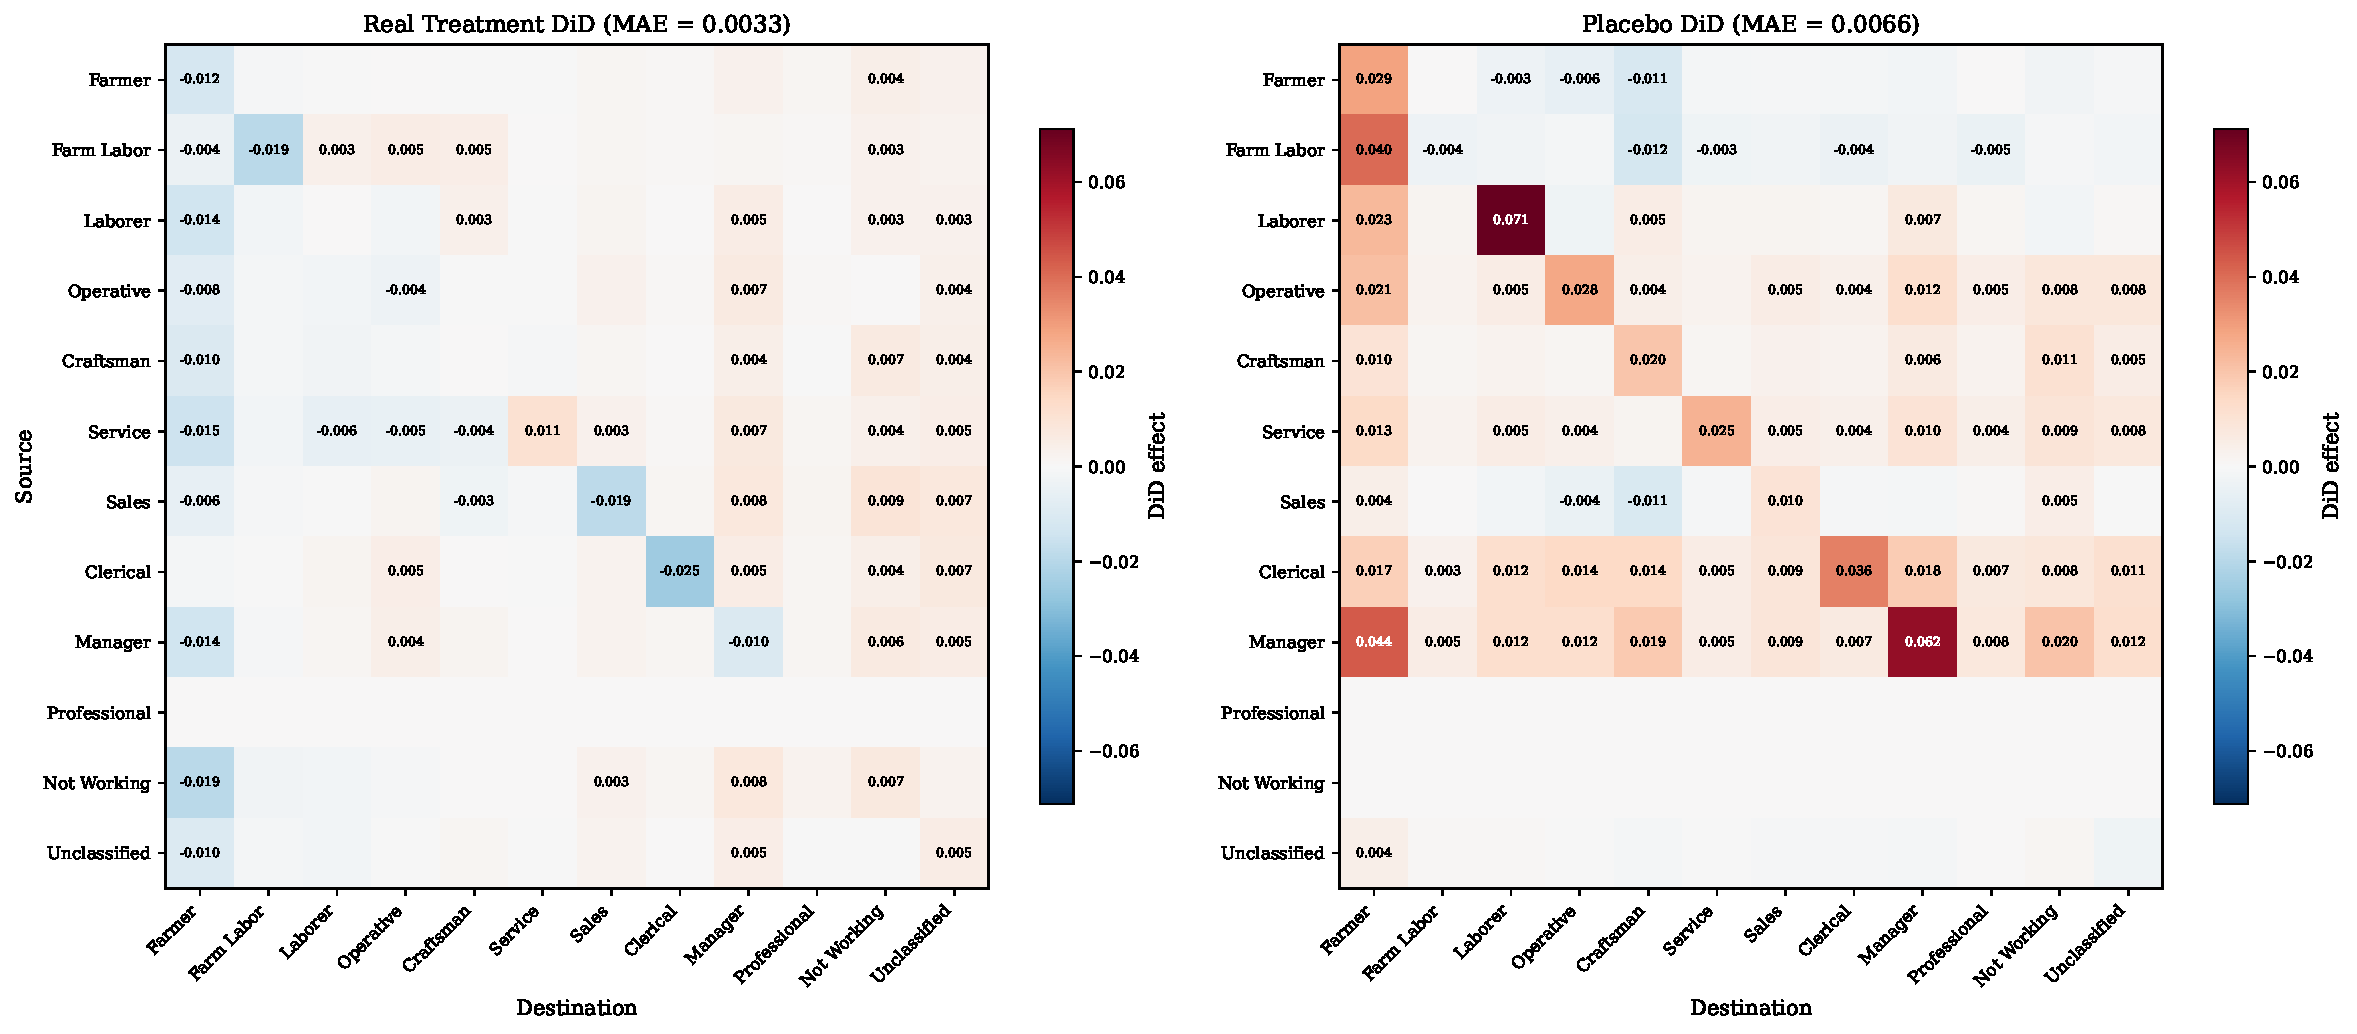
\includegraphics[width=\textwidth]{figures/placebo_comparison.pdf}
    \caption{Real treatment (left) vs.\ placebo (right) DiD transition matrices. The treatment shows structured farmer avoidance (negative Farmer column) and skill-match displacement channels. The placebo shows the opposite pattern (positive Farmer column), confirming that treatment effects reflect TVA-induced changes, not method artifacts.}
    \label{fig:placebo}
\end{figure}

The placebo DiD produces the \textit{opposite} sign pattern in the Farmer column (positive rather than negative), and the treatment-specific skill-match channels (farm labor $\to$ operative, farm labor $\to$ craftsman) do not appear. The treatment effects reflect TVA-induced structural changes, not artifacts of the estimation method or geographic composition.

\subsection{Weight-Space Analysis}

Beyond statistical extraction, we analyze the treatment effect directly in the model's weight space. SVD decomposition of the double-differenced adapter weight matrices reveals that the treatment effect is strikingly low-rank: across 18 LoRA modules, the top singular value captures 48--98\% of total energy. FFN layers show the highest concentration (94--98\%), implying that TVA-induced structural transformation operated primarily along a single direction in the model's representation space. Full SVD results appear in \Cref{app:svd}.

\begin{figure}[H]
    \centering
    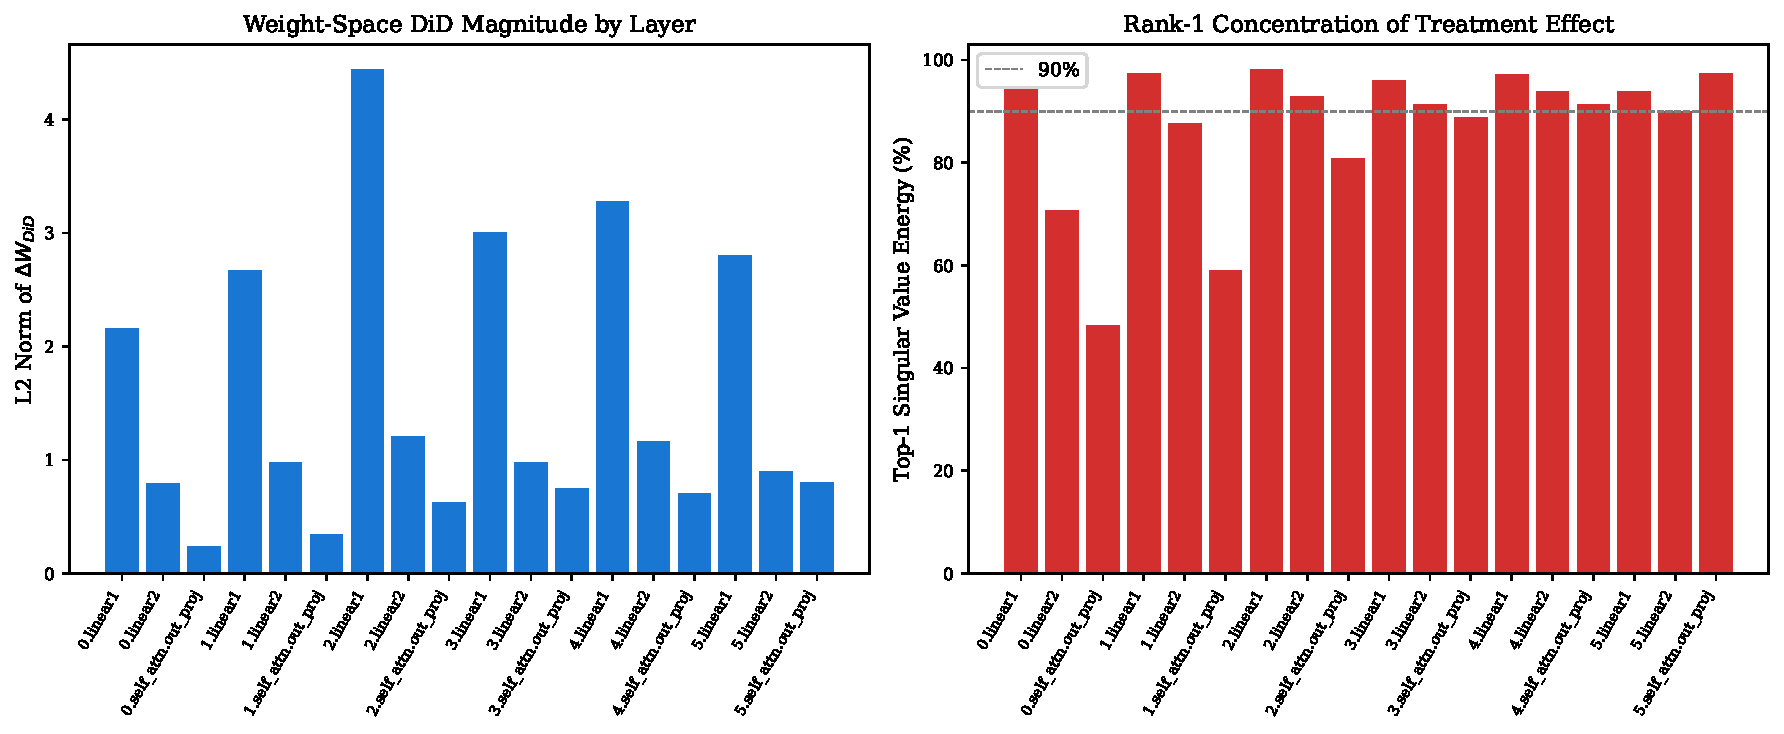
\includegraphics[width=\textwidth]{figures/svd_spectrum.pdf}
    \caption{Weight-space DiD analysis. Left: L2 norm of the double-differenced adapter weights by layer. Right: rank-1 energy concentration. Most layers concentrate $>$90\% of the treatment signal in a single direction, consistent with a dominant structural force (cheap electricity $\to$ factory employment).}
    \label{fig:svd_spectrum}
\end{figure}

\subsection{Linkage Selection}

Record linkage introduces potential selection bias if linkage rates differ between TVA and control counties \citep{abramitzky2021, heckman1998}. Three features mitigate this concern.

First, baseline characteristics are well-balanced on age (33.2 years in both groups) and broadly similar on other observables (\Cref{tab:sample}). The main compositional difference---higher agricultural share in TVA counties (53.9\% vs.\ 45.2\%)---is expected given the program's target population and is the variation that drives identification.

Second, if mobile workers---those most affected by the TVA---are harder to link across censuses, our estimates \textit{understate} the true treatment effects. Workers who migrated between counties in response to TVA-induced industrialization are less likely to appear in the linked sample, since the probabilistic linkage relies on name-age-birthplace matches that degrade when individuals move to new locations and change household compositions. This creates a selection bias \textit{toward zero}: the most-affected workers are systematically missing, and the linked sample over-represents stayers. The direction of bias is therefore conservative---our estimates are intent-to-treat (ITT) by 1920 county of residence, not treatment-on-the-treated.

Third, the pattern of results argues against a linkage-driven artifact. If differential linkage were generating spurious effects, we would expect the pattern to correlate with linkage difficulty rather than with economic mechanisms. The farm laborer $\to$ operative and farm laborer $\to$ craftsman transitions are economically specific (they involve particular skill-match pathways) rather than reflecting a generic ``more mobile workers drop out'' bias. Moreover, the placebo test splits the same linked sample by geographic assignment and produces the \textit{opposite} pattern, confirming that the treatment effects do not arise from the linkage process.

\subsection{Sensitivity to Identification Assumptions}

\textbf{TVA timing.} The TVA was established in 1933, and major dam construction continued through 1945. Our pre-treatment period (1920$\to$1930) predates TVA establishment, and our post-treatment period (1930$\to$1940) captures the first 7 years of TVA operation. The 1930 census was collected before TVA existence, but the 1940 census captured workers who had already been exposed to TVA-related economic changes for up to 7 years. The fact that we detect economically meaningful transition effects in this relatively short window suggests that labor market restructuring was rapid, consistent with the ``big push'' interpretation of \citet{kline2014}.

\textbf{Alternative control group.} Our main control group includes non-TVA counties within TVA-region states (e.g., non-TVA counties in Tennessee, Alabama, Kentucky). These counties may experience indirect TVA effects through electricity access, labor market spillovers, or state-level fiscal complementarities. To test sensitivity, we re-estimate the full four-adapter pipeline using only the 9 non-TVA states as controls (\num{1300975} individuals), excluding all TVA-region states entirely.

The alternative-control DiD matrix correlates 0.86 with the baseline results (MAE = 0.004). The core patterns replicate: farm labor stay-rate disruption ($-5.7$pp vs.\ $-1.9$pp baseline), Lewis channel displacements (farm labor $\to$ operative: $+1.6$pp, farm labor $\to$ craftsman: $+1.6$pp), and broad manager-entry increases. Effects are generally larger in magnitude, consistent with the baseline control group experiencing partial TVA spillovers that attenuate our main estimates toward zero. The results are robust to this restrictive control group definition.

\textbf{LoRA rank sensitivity.} The transformer's LoRA adapters use rank $r = 8$ in the baseline. We test sensitivity to rank by re-running the alternative control group pipeline at $r \in \{4, 8, 16\}$. All three rank settings produce DiD matrices that correlate $> 0.80$ with the baseline (all-control, $r = 8$) results: $r = 4$ yields 0.80, $r = 8$ yields 0.86, and $r = 16$ yields 0.74. Cross-rank correlations range from 0.76 to 0.83. The core pattern of farm labor disruption and manufacturing absorption persists across ranks, though individual cell magnitudes vary. The moderate sensitivity suggests that the broad qualitative story is robust but precise point estimates should be interpreted with appropriate uncertainty.

\textbf{Aggregation weighting.} We aggregate from 575 life-state tokens to 12 occupation categories using equal weighting across tokens within each category. This means that a rare life-state token (e.g., Farmer\_Mining\_Wid\_6k+) receives the same weight as a common one (e.g., Farmer\_Agr\_Mar\_12k). An alternative approach would weight by population frequency (e.g., the pooled 1920 composition), yielding a population-representative average. The equal-weight and population-weight estimates may differ for occupations with substantial within-category heterogeneity. We report equal-weight results throughout and note that the frequency benchmark implicitly uses population weighting, providing a complementary perspective.


%% ============================================================
%% 7. CONCLUSION
%% ============================================================
\section{Conclusion}
\label{sec:conclusion}

The TVA did not simply shrink agriculture and grow manufacturing. It reorganized the entire landscape of career possibilities in the Tennessee Valley. Farm laborers shifted to factory floors. Farmers moved into management. Workers across the occupation structure stopped entering agriculture. These are not regression coefficients---they are specific, named transitions between specific occupations, each with different implications for skills, earnings, and adjustment costs.

We recover these pathways by estimating an occupation-level DiD transition matrix from 2.5 million linked census records. The main contribution is the \textit{estimand}: transition matrices as first-class treatment effects. The specific estimator---whether a transformer or raw frequency counts---matters less than the question being answered. Both methods agree on the dominant patterns. Where they disagree (the Farmer destination column), the disagreement itself is informative.

Several limitations deserve attention. First, the three-period design provides only one pre-treatment transition. Extension to 1910--1920 links would give a second pre-period and a proper event study. The near-zero pre-trends (MAE = 0.0002) support parallel trends but cannot rule out differential Depression-era shocks.

Second, non-TVA counties within TVA states may experience spillovers. The alternative control group using only non-TVA states correlates 0.86 with baseline results but produces systematically larger effects, suggesting that the main estimates are attenuated by partial spillover contamination.

Third, the transformer and frequency estimators diverge on some cells---particularly the Farmer column, where the transformer shows uniform avoidance and the frequency estimator shows mixed signs. This reflects genuine differences in what the estimators condition on (the transformer uses life-state tokens encoding occupation, industry, marital status, and children; the frequency estimator uses occupation alone). Neither is ``right''---they answer slightly different questions.

Fourth, we pool races despite stark TVA-era occupational segregation. Black workers (7.4\% of TVA counties) faced different transition constraints than White workers. Race-specific transition matrices would require adequate sample sizes in each race $\times$ treatment $\times$ period $\times$ occupation cell---a demanding requirement.

Fifth, linkage selection deserves scrutiny. The IPUMS MLP v2.0 links approximately 60--70\% of the male population, and linkability depends on name stability, consistent age reporting, and geographic persistence---traits correlated with socioeconomic status and mobility. More mobile workers (who may be most affected by TVA) are harder to link, potentially attenuating our ITT estimates. The direction of bias is likely conservative: if TVA-induced movers are disproportionately excluded, the observed transition effects understate the true reallocation. A formal test would compare linkage rates by TVA status $\times$ 1920 occupation; aggregate linkage rates are similar across TVA and control counties, but occupation-specific linkage differences remain unquantified.

Sixth, our ITT design assigns treatment by 1920 county of residence. Workers who migrated in response to TVA-induced industrialization contribute to the treatment effect, but we cannot separate migration from occupational transition.

These are real limitations. They do not diminish the main point: \textit{transition matrices are the natural treatment effect for policy that reshapes career paths}. When we ask how place-based industrial policy affects workers, the answer is not a number---it is a matrix. That matrix reveals the distributional anatomy that aggregate analysis conceals.

The approach generalizes. Trade shocks that displace manufacturing workers \citep{autor2013}, automation that eliminates routine tasks \citep{autor2003, deming2020}, job training programs, immigration shocks---in each case, the standard treatment effect compresses the entire reallocation story into one coefficient. The transition matrix tells the rest. For any setting with linked panel data and a credible DiD design, the question ``who moved where?'' is answerable. Future work could link transition estimates to occupation-level earnings to quantify the welfare implications of each pathway \citep{hsieh2019}.


%% ============================================================
%% BIBLIOGRAPHY
%% ============================================================
\newpage

\noindent\textbf{Project Repository:} \url{https://github.com/SocialCatalystLab/ape-papers}

\noindent\textbf{Contributors:} @SocialCatalystLab

\label{apep_main_text_end}

\bibliography{references}

\newpage
\appendix

%% ============================================================
%% APPENDIX A: Model Architecture
%% ============================================================
\section{Model Architecture and Training}
\label{app:model}

\begin{table}[H]
\centering
\caption{Model Configuration}
\label{tab:config}
\begin{tabular}{lr}
\toprule
Parameter & Value \\
\midrule
Vocabulary size & 573 life-state + 3 special (NW, UNCL, PAD) = 576 \\
Embedding dimension ($d$) & 128 \\
Decoder layers & 6 \\
Attention heads & 2 \\
FFN dimension & 512 \\
Dropout & 0.05 \\
Total parameters & \num{1342017} \\
\addlinespace
\textit{Pre-training:} & \\
\quad Training sequences & \num{10851318} \\
\quad Steps & \num{15000} \\
\quad Batch size & 512 \\
\quad Learning rate & $5 \times 10^{-4}$ \\
\quad Best val loss & 3.89 (step \num{8500}) \\
\quad Temporal masking & Position 1 zeroed \\
\addlinespace
\textit{LoRA fine-tuning (per adapter):} & \\
\quad Rank ($r$) & 8 \\
\quad Alpha ($\alpha$) & 16.0 \\
\quad LoRA modules & 18 (all projections) \\
\quad Trainable parameters & \num{73728} (5.2\%) \\
\quad Steps & \num{1500} \\
\quad Batch size & 256 \\
\quad Learning rate & $1 \times 10^{-4}$ \\
\bottomrule
\end{tabular}
\end{table}

The architecture follows CAREER \citep{vafa2022} with modifications for causal inference:
\begin{itemize}
    \item \textbf{Token embedding:} Each life-state token maps to a 128-dimensional embedding encoding occupation, industry, marital status, and children jointly.
    \item \textbf{Covariate side-embeddings:} Census year, age bin, race, and sex each get separate embedding tables, \textit{added} (not concatenated) to the token embedding.
    \item \textbf{Causal decoder:} 6 pre-norm transformer layers with 2 attention heads and 512-dimensional FFN. Causal masking ensures each position attends only to current and previous tokens.
    \item \textbf{Two-stage prediction head:} Sigmoid stay probability $P(\text{stay})$ plus softmax over transition destinations, allocating capacity to the informative off-diagonal transitions.
\end{itemize}

\subsection{Adapter Convergence}

\begin{table}[H]
\centering
\caption{Four-Adapter Training Summary}
\label{tab:adapter_training}
\begin{tabular}{lrrrr}
\toprule
Adapter & $N$ Individuals & Best Val Loss & Training Time & Steps \\
\midrule
TVA-pre & \num{318335} & 3.32 & 50s & \num{1500} \\
TVA-post & \num{318335} & 3.28 & 50s & \num{1500} \\
Control-pre & \num{2193640} & 3.44 & 78s & \num{1500} \\
Control-post & \num{2193640} & 3.32 & 79s & \num{1500} \\
\bottomrule
\end{tabular}
\end{table}


%% ============================================================
%% APPENDIX B: Synthetic Validation
%% ============================================================
\section{Synthetic Validation}
\label{app:validation}

We validate the method on four synthetic data-generating processes with known ground-truth treatment effects.

\begin{table}[H]
\centering
\caption{Synthetic Validation Results}
\label{tab:synthetic}
\begin{threeparttable}
\begin{tabular}{lcccccc}
\toprule
DGP & Tokens & Parameters & Steps & Control MAE & Effect Recovery & Time \\
\midrule
1 (Sanity) & 3+pad & 18K & 2,000 & 0.005 & Ratio 1.07 & 26s \\
2 (TVA lite) & 5+pad & 103K & 3,000 & 0.002 & Ratio 1.07 & 102s \\
2-null & 5+pad & 103K & 3,000 & 0.002 & Max spurious 1.5pp & 104s \\
3 (Census) & 33+pad & 545K & 6,000 & 0.005 & 3/3 top cells correct & 13min \\
\bottomrule
\end{tabular}
\begin{tablenotes}[flushleft]
\small
\item Notes: Control MAE measures average absolute difference between model-extracted and true transition matrices. The null DGP (no treatment effect) produces maximum spurious effects of 1.5pp, confirming low false positive rates.
\end{tablenotes}
\end{threeparttable}
\end{table}


%% ============================================================
%% APPENDIX C: Weight-Space SVD
%% ============================================================
\section{Weight-Space SVD Details}
\label{app:svd}

\begin{table}[H]
\centering
\caption{Weight-Space DiD SVD by Layer}
\label{tab:svd}
\begin{threeparttable}
\begin{tabular}{lccc}
\toprule
Layer & L2 Norm & Top-3 $\sigma$ & Top-1 Energy \\
\midrule
0.linear1 & 2.16 & 2.10, 0.50, 0.12 & 94\% \\
0.linear2 & 0.79 & 0.67, 0.41, 0.12 & 71\% \\
0.self\_attn.out\_proj & 0.24 & 0.17, 0.14, 0.09 & 48\% \\
\addlinespace
1.linear1 & 2.67 & 2.64, 0.43, 0.09 & 97\% \\
1.linear2 & 0.98 & 0.92, 0.32, 0.11 & 88\% \\
1.self\_attn.out\_proj & 0.34 & 0.26, 0.17, 0.10 & 59\% \\
\addlinespace
2.linear1 & 4.44 & 4.40, 0.60, 0.13 & 98\% \\
2.linear2 & 1.20 & 1.16, 0.29, 0.14 & 93\% \\
2.self\_attn.out\_proj & 0.62 & 0.56, 0.25, 0.08 & 81\% \\
\addlinespace
3.linear1 & 3.01 & 2.95, 0.58, 0.16 & 96\% \\
3.linear2 & 0.98 & 0.93, 0.25, 0.14 & 91\% \\
3.self\_attn.out\_proj & 0.75 & 0.71, 0.20, 0.11 & 89\% \\
\addlinespace
4.linear1 & 3.27 & 3.23, 0.54, 0.14 & 97\% \\
4.linear2 & 1.16 & 1.12, 0.25, 0.14 & 94\% \\
4.self\_attn.out\_proj & 0.71 & 0.68, 0.19, 0.08 & 91\% \\
\addlinespace
5.linear1 & 2.80 & 2.72, 0.68, 0.13 & 94\% \\
5.linear2 & 0.90 & 0.85, 0.24, 0.14 & 90\% \\
5.self\_attn.out\_proj & 0.80 & 0.79, 0.10, 0.07 & 97\% \\
\bottomrule
\end{tabular}
\begin{tablenotes}[flushleft]
\small
\item Notes: L2 norm of $\Delta W^{\text{DiD}}$ for each LoRA module. FFN layers (linear1) carry the largest treatment effects. Top-1 energy exceeds 90\% in most layers, indicating near-rank-1 treatment structure.
\end{tablenotes}
\end{threeparttable}
\end{table}


%% ============================================================
%% APPENDIX D: Data Construction
%% ============================================================
\section{Data Construction Details}
\label{app:data}

\subsection{MLP Crosswalk}

The IPUMS MLP crosswalk v2.0 contains \num{175649924} potential links across census waves from 1850 to 1950. We restrict to males aged 18--65 in 1920 residing in TVA or control counties across 16 states, yielding \num{2511975} linked career sequences.

\subsection{TVA County Definitions}

We identify 164 TVA counties across 7 states using IPUMS COUNTYICP codes, following \citet{kline2014}.

\begin{table}[H]
\centering
\caption{TVA Counties by State}
\label{tab:tva_counties}
\begin{tabular}{lr}
\toprule
State & $N$ Counties \\
\midrule
Alabama & 20 \\
Georgia & 8 \\
Kentucky & 12 \\
Mississippi & 15 \\
North Carolina & 11 \\
Tennessee & 86 \\
Virginia & 12 \\
\midrule
Total & 164 \\
\bottomrule
\end{tabular}
\end{table}




\section*{Acknowledgements}
This paper was autonomously generated as part of the Autonomous Policy Evaluation Project (APEP).

\noindent\textbf{Contributors:} @SocialCatalystLab

\noindent\textbf{First Contributor:} \url{https://github.com/SocialCatalystLab}

\noindent\textbf{Project Repository:} \url{https://github.com/SocialCatalystLab/ape-papers}

\end{document}
